\documentclass[12pt,a4paper]{article}

\usepackage{amsmath, amssymb}
\usepackage[utf8]{inputenc}
\usepackage[english]{babel}
\usepackage{graphicx}
\usepackage[margin=0.5in]{geometry}
\usepackage{float}

\graphicspath{{fig/}}


\begin{document}

\section{Writing Controller Code}
This section blablabla
\subsection{Level 1}
The code equivalent to the Simulink block gave similar results which can be seen in Figure \ref{fig:task2_traj} and Figure \ref{fig:task2_pos}. A sampling time of 10 ms was used for the code. Different sampling times were tested and it was noticed that when using a lower sampling time the impact on the trajectory planner increased. When a lower sampling time is used the change of acceleration is missed by a few milliseconds and therefore impact the velocity and position. This gives the difference in the position of the motor which is seen in Figure \ref{fig:task2_pos}.
\begin{figure}[h]
	\begin{center}
	
		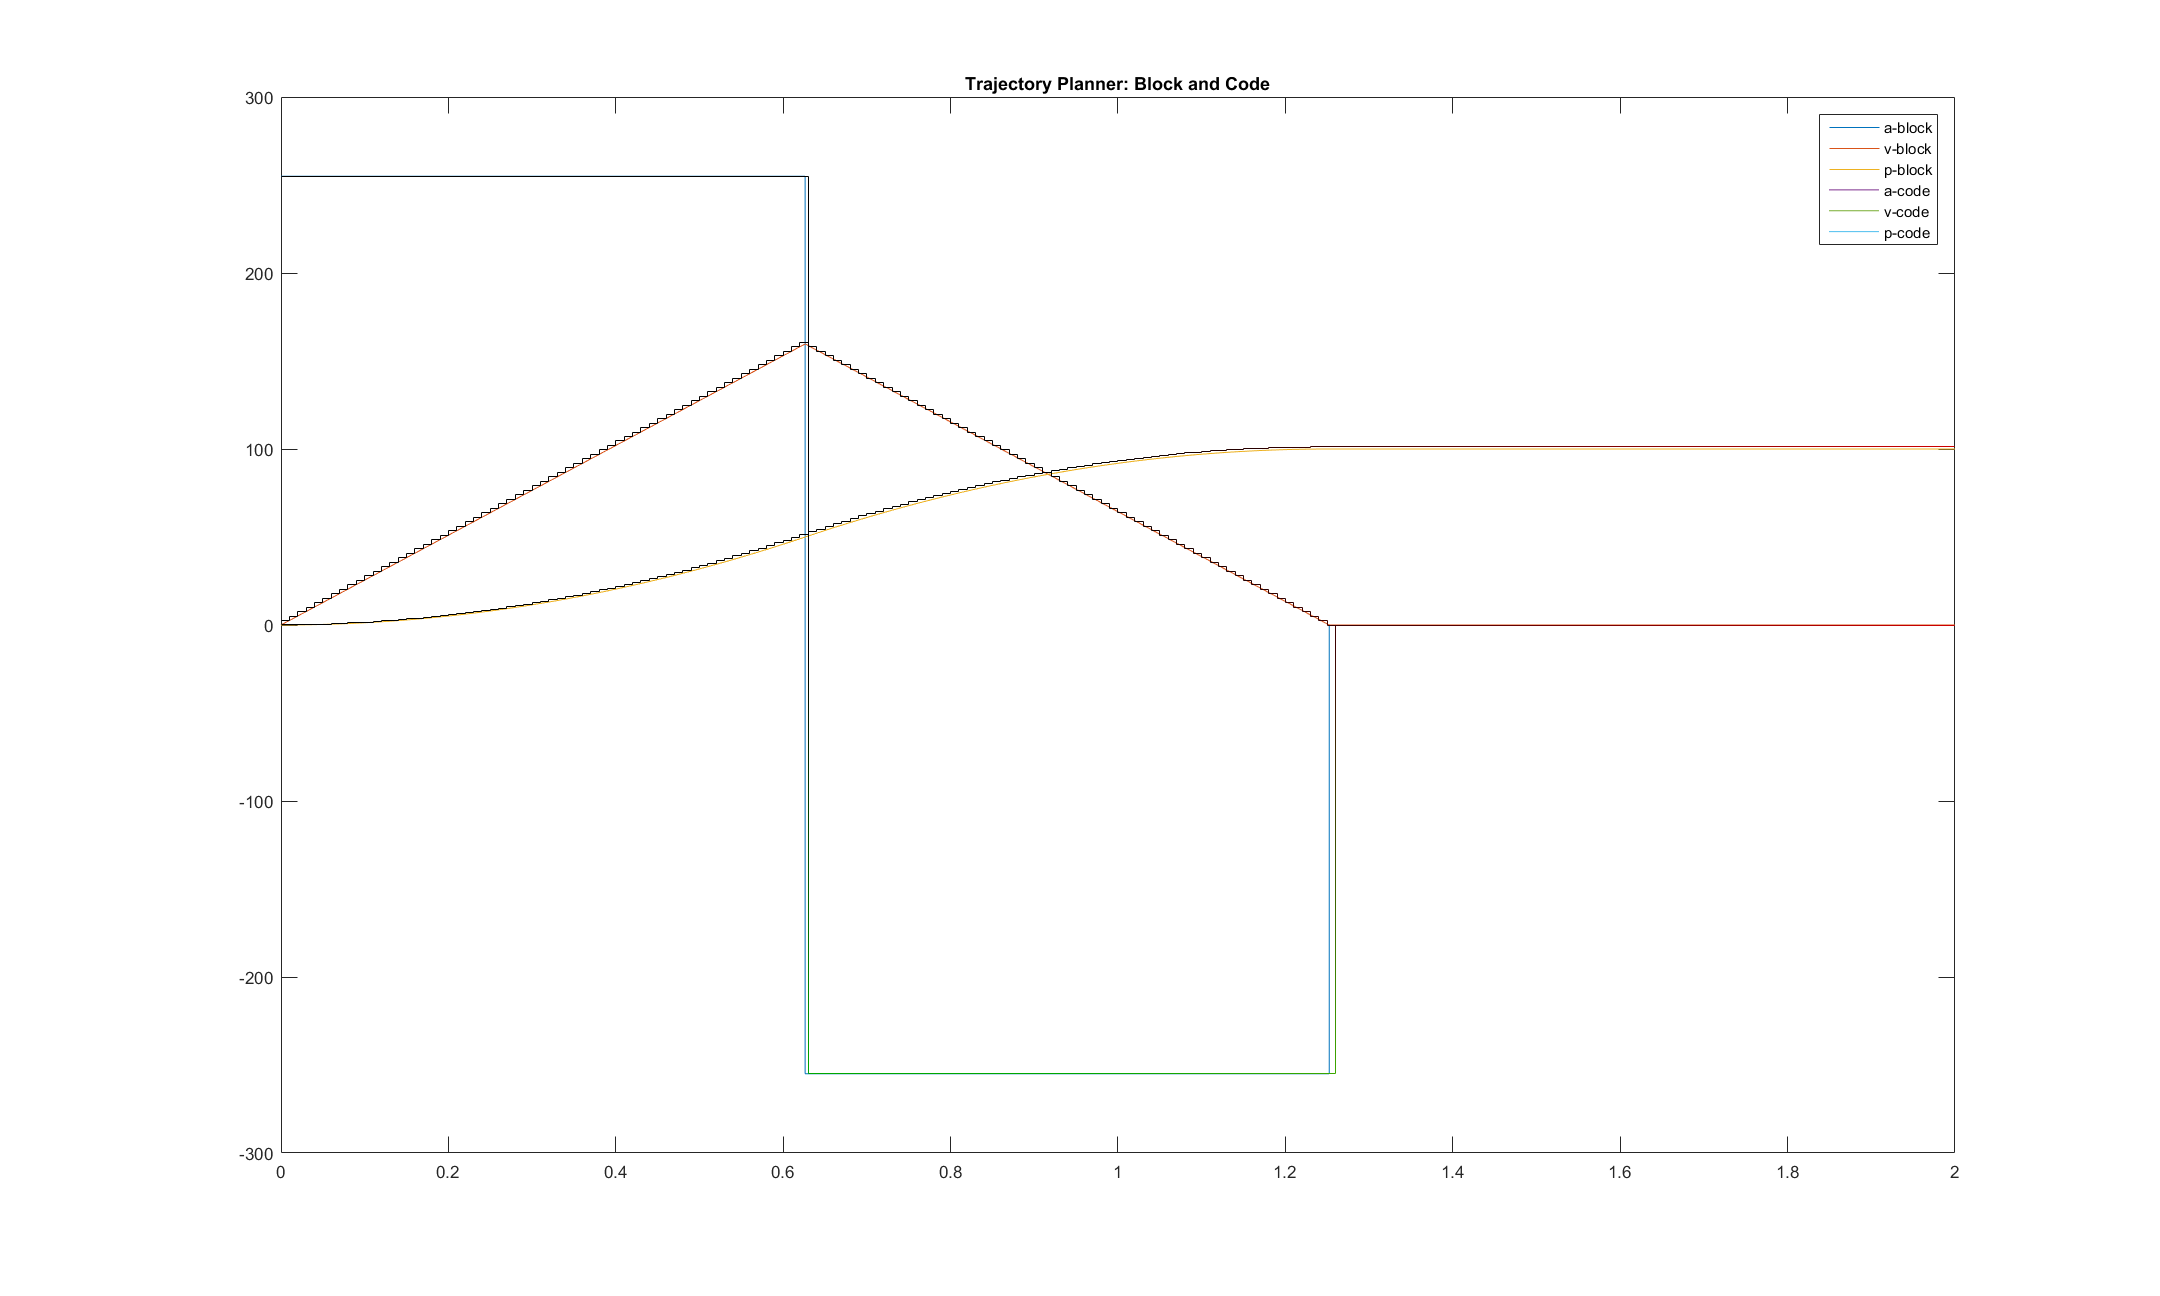
\includegraphics[scale=0.2]{task2_traj.png}
		\caption{Trajectory planner signal comparison}
		\label{fig:task2_traj}
	\end{center}
\end{figure}



\begin{figure}[h]
	\begin{center}
	
		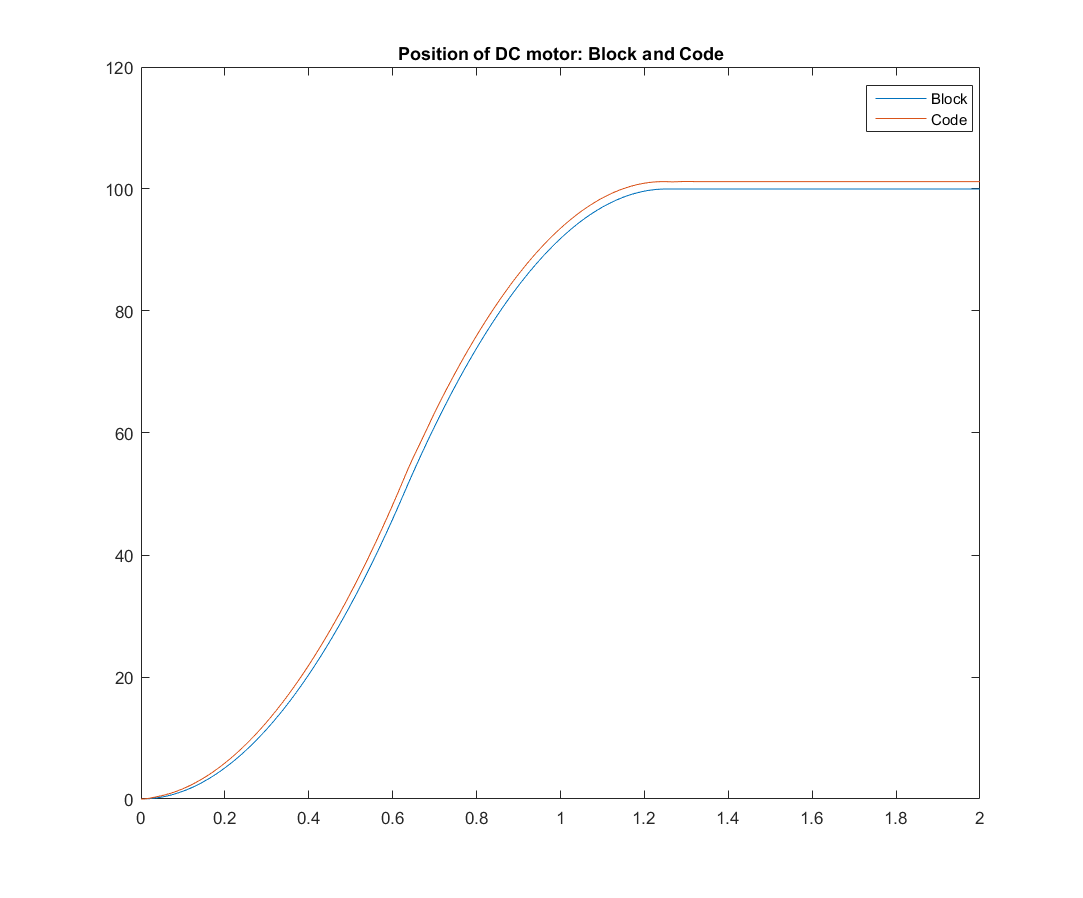
\includegraphics[scale=0.2]{task2_position.png}
		\caption{Motor position comparison}
		\label{fig:task2_pos}
	\end{center}
\end{figure}





\end{document}
